\documentclass{article}
\usepackage{enumitem}
\usepackage{graphicx}
\usepackage{subcaption}
\usepackage{tikz}


\begin{document}

\section*{3D Reconstruction and dimention measurement}
Talk about how the task applied in reality

\subsection*{3D Reconstruction Procedures}
In the order to reconstruct a 3D model of a specific object, \textbf{Draven} rotate around it capturing a video to be saved as input images, and yet through a Structure From Motion algorithm it produces a dense model of object then adds a texture to the model, as specsified in Figure \ref{fig:reconstruction}.

\begin{figure}[h]
  \centering
  \begin{tikzpicture}
    % First figure
    \node[draw, rectangle, blue] (figure1) at (0,2) {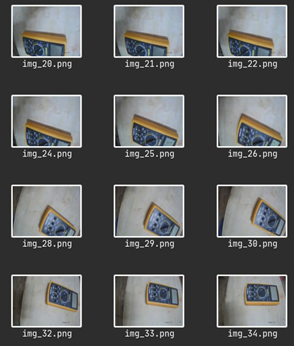
\includegraphics[width=0.3\textwidth]{3d_task_figure2/input_images.png}};
    \node[above=65pt, text width=100pt,align=center] at (figure1) {Samples from input images};
  
    % Second figure
    \node[draw, rectangle, blue] (figure2) at (4,2) {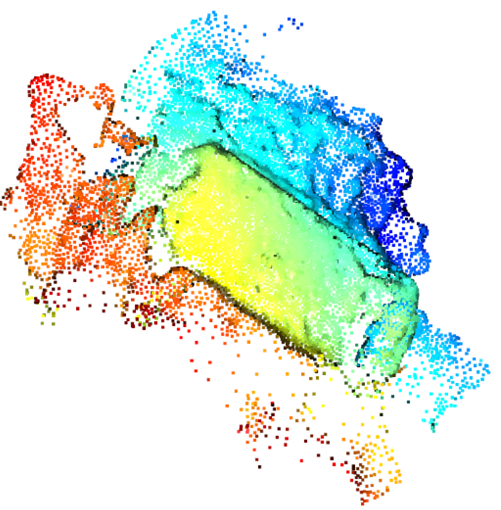
\includegraphics[width=0.25\textwidth]{3d_task_figure2/dense.png}};
    \node[above=50pt, text width=100pt,align=center] at (figure2) {Dense reconstruction Output};
  
    % Third figure
    \node[draw, rectangle, blue] (figure3) at (8,4) {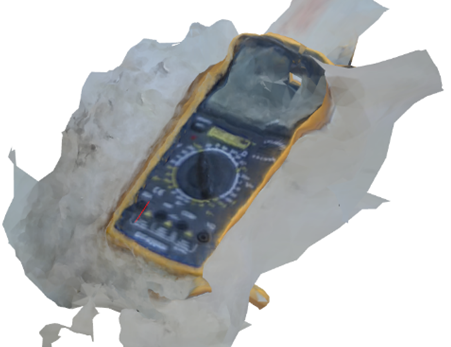
\includegraphics[width=0.27\textwidth]{3d_task_figure2/output1.png}};
    \node[above=40pt,text width=100pt,align=center] at (figure3) {Texture Output from different views};
  
    % third figure
    \node[draw, rectangle, blue] (figure4) at (8,0) {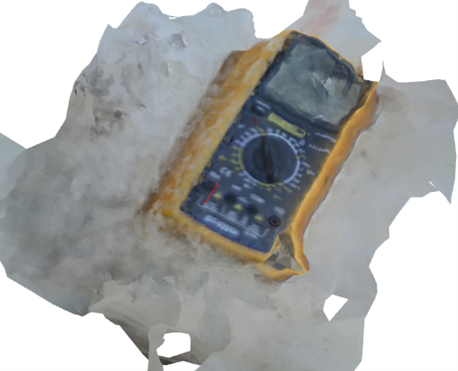
\includegraphics[width=0.27\textwidth]{3d_task_figure2/output2.png}};
    
    % Arrow between figures
    \draw[->, line width=1.3pt, blue] (figure1) -- (figure2);
    \draw[->, line width=1.3pt, blue] (figure2) -- (figure3);
    \draw[->, line width=1.3pt, blue] (figure2) -- (figure4);
  \end{tikzpicture}
  \caption{Reconstruction process}
  \label{fig:reconstruction}
  \end{figure}

% \subsection*{Process Overview}
% \begin{itemize}[label=-]
%   \item SfM involves several fundamental steps, including feature extraction, matching, camera pose estimation, and dense reconstruction.
%   \item Feature points are identified in the images and matched across different viewpoints to establish correspondences.
% \end{itemize}

\subsection*{Dimentions measurement procedures}
To measure the required dimentions, \textbf{Draven} measure a specsified dimention input from user during runtime through a GUI using Streo Camera Calibration, then it can be saved as a reference on the 3D model for other dimentions measurement, as specsified in Figure \ref{fig:measurement}.

\begin{figure}[h]
  \centering
\begin{tikzpicture}
  % First figure
  \node[draw, rectangle, blue] (figure1) at (0,0) {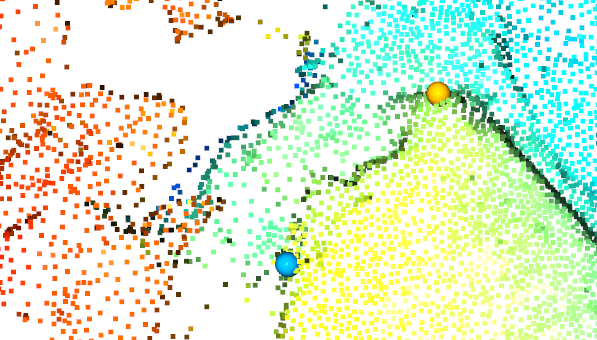
\includegraphics[width=0.25\textwidth]{3d_task_figure1/reference.png}};
  \node[above=40pt, text width=3cm,align=center] at (figure1) {Known size reference};

  % Second figure
  \node[draw, rectangle, blue] (figure2) at (4,0) {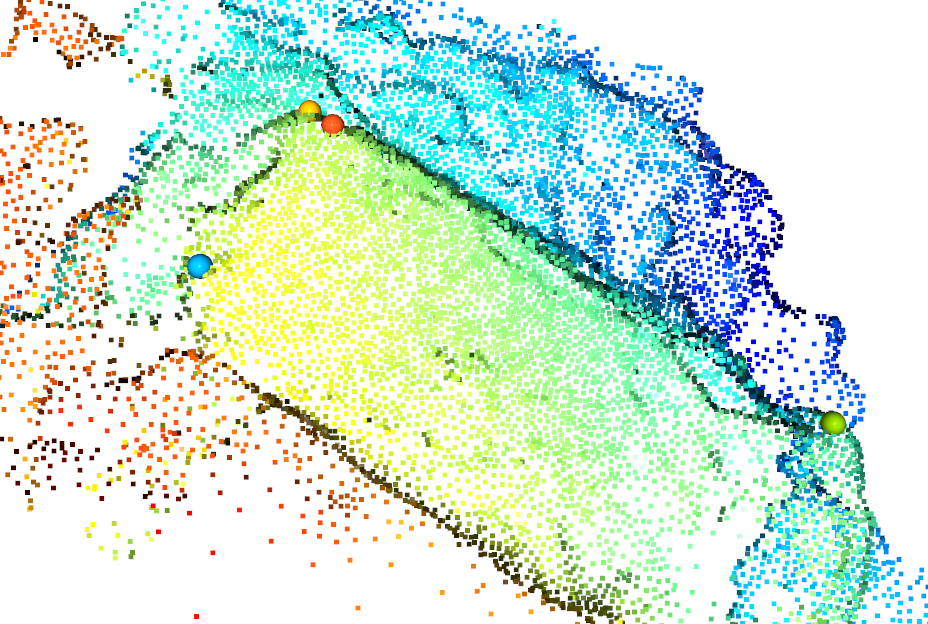
\includegraphics[width=0.25\textwidth]{3d_task_figure1/distance to be measured.png}};
  \node[above=40pt, text width=100pt,align=center] at (figure2) {Distance to be measured};

  % Third figure
  \node[draw, rectangle, blue] (figure3) at (8,0) {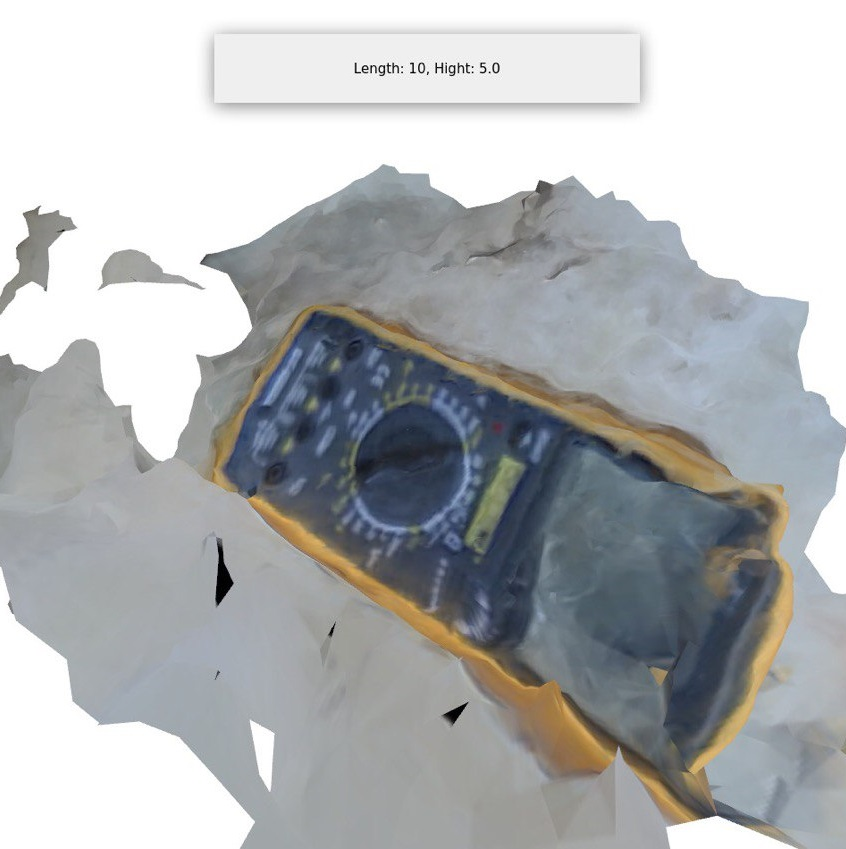
\includegraphics[width=0.32\textwidth]{3d_task_figure1/measurement_output.jpg}};
  \node[above=60pt,text width=100pt,align=center] at (figure3) {Measured distance labeled on the model};

  % Arrow between figures
  \draw[->, line width=1.3pt, blue] (figure1) -- (figure2);
  \draw[->, line width=1.3pt, blue] (figure2) -- (figure3);

\end{tikzpicture}
\caption{Measuring process}
\label{fig:measurement}
\end{figure}
\end{document}
